\documentclass[12pt, letterpaper]{article}

\usepackage{amsmath} % needed for including equations
\usepackage[margin=1in]{geometry} % sets the margins to 1in
\usepackage{graphicx} % needed for figures
\graphicspath{{./figures/}} % allows figures to be placed in a different folder
\usepackage[hang,small,bf]{caption} % sets the style on the figure captions
\usepackage{epstopdf} % converts eps files to pdf to display in the latex document



\begin{document}

\begin{titlepage}

\begin{center}

\vspace*{\fill}

\vspace{0.5in}

% Insert your title here
{ \LARGE \bfseries Simultaneous Collaborative UAV Exploration and Mapping In GPS Denied Environments}\\[.25in]

\large
by\\[.25 in]
% Change your name here
Jacob M. Olson\\[1in]

A prospectus submitted to the faculty of\\
Department of Mechanical Engineering\\
Brigham Young University

\vspace{1in}

\today

\vspace*{\fill}

\end{center}

\end{titlepage}

\thispagestyle{empty}

\begin{center}
\vspace*{\fill}

\begin{figure}[htbp] %  figure placement: here, top, bottom, or page
   \centering
   
\includegraphics[width=2.5in]{byume_logo_clear.jpg} 
\end{figure}

\vspace{0.5in}

\Large{Prospectus Approval}\\[0.5in]

\end{center}

\hspace*{.47in}
\begin{minipage}[c]{5.25in}

\normalsize

Prospectus submitted by:

\vspace{.5in}

\makebox[2in]{\hrulefill} \hspace{1in} \makebox[2in]{\hrulefill}

% Change your name here
\parbox[b]{3in}{Jacob Olson} \, Date
\vspace{0.5in}

This prospectus has been approved by each member of the Graduate Committee:
\vspace{0.5in}

\makebox[2in]{\hrulefill} \hspace{1in} \makebox[2in]{\hrulefill}

\parbox[b]{3in}{Committee Member - Chair} \, Date
\vspace{0.4in}

\makebox[2in]{\hrulefill} \hspace{1in} \makebox[2in]{\hrulefill}

\parbox[b]{3in}{Committee Member} \, Date
\vspace{0.4in}

\makebox[2in]{\hrulefill} \hspace{1in} \makebox[2in]{\hrulefill}

\parbox[b]{3in}{Committee Member} \, Date

\end{minipage}

\vspace*{\fill}

\pagebreak

\setcounter{page}{1}

\section{Problem Statement}
During a disaster such as an earthquake or fire, buildings are often left structurally unsound. Sending in a human team to inspect the building can unnecessarily put human lives at risk. This project seeks to minimize the problem by sending in a swarm of intelligent unmanned aerial vehicles (UAVs) deployed from a larger, tethered UAV shown in Figure \ref{fig:sentinel_survey}. The swarm is able to map a building, scan for damaged structures, and identify the source of a fire to determine the level of damage and whether it is safe to send in first responders.

\begin{figure}[h] %  figure placement: here, top,  bottom, or page
	\centering
	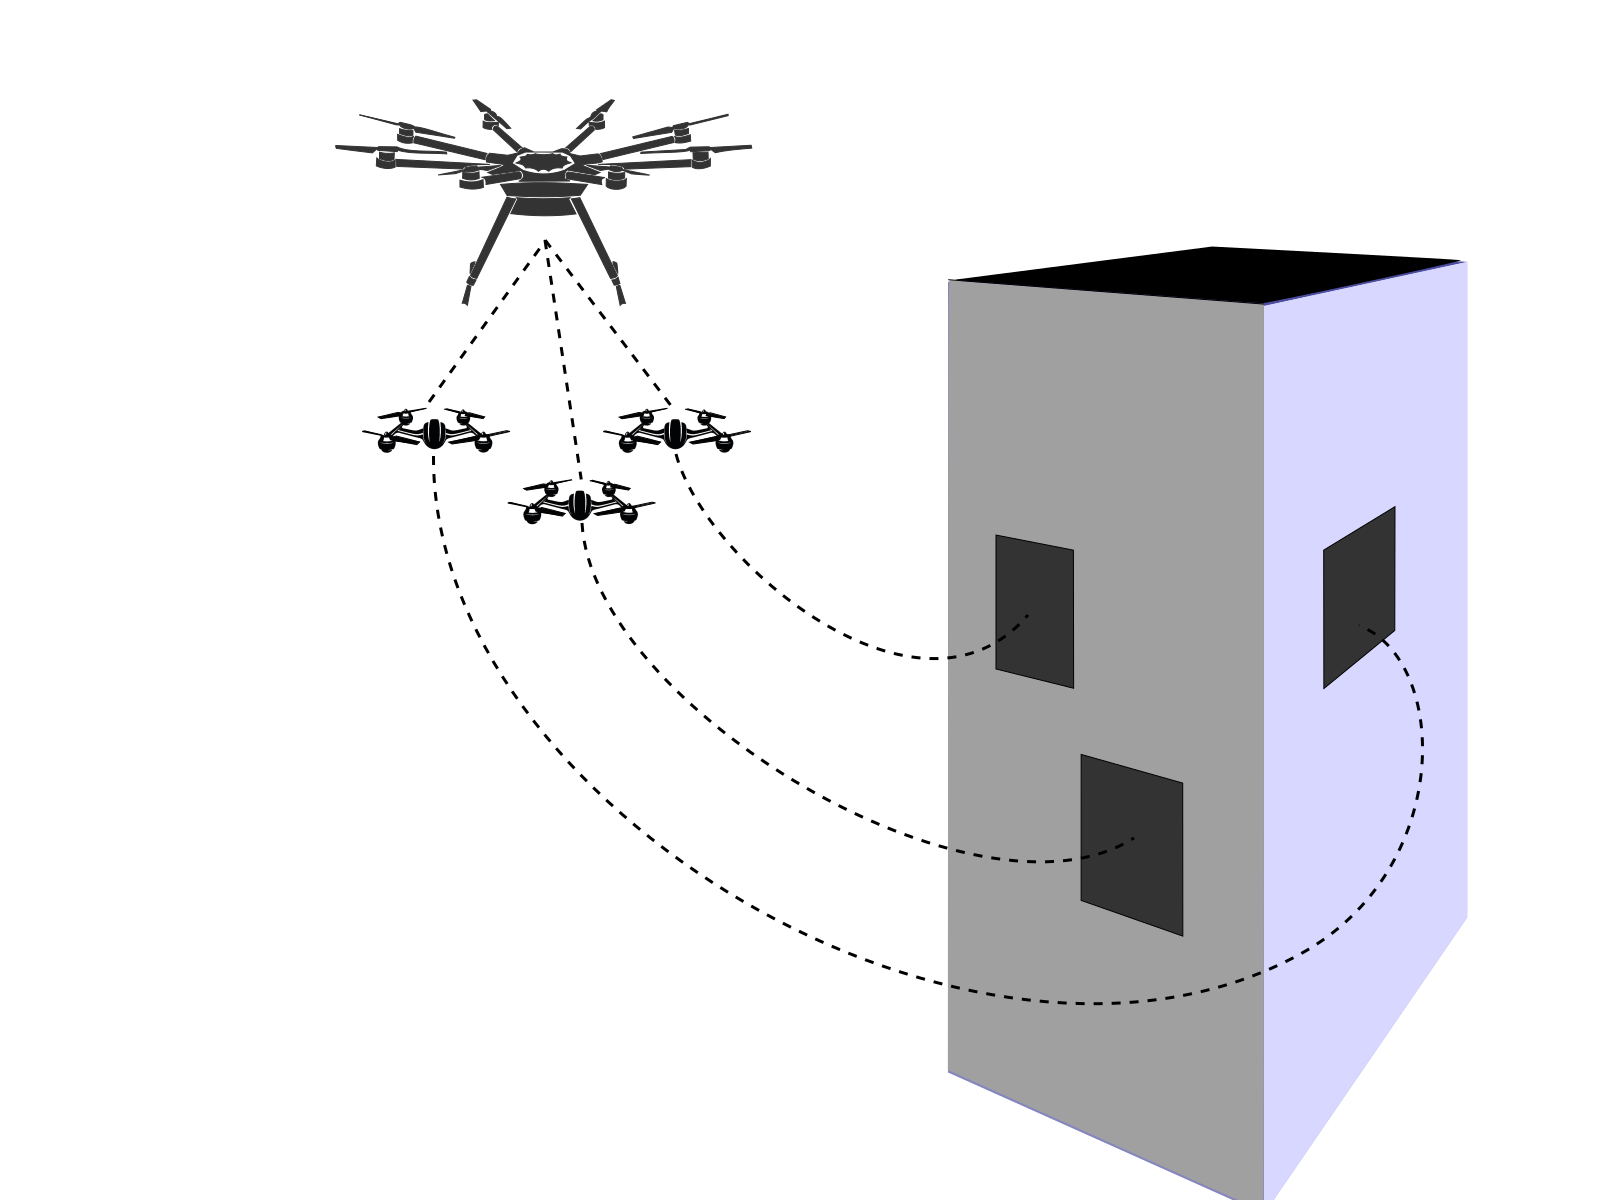
\includegraphics[trim = 0mm 0mm 0mm 0mm,clip,width=3in]{survey_drone_illustration.png}
	\caption{Survey UAVs deploy from Sentinel UAV to map a GPS-Denied area}
	\label{fig:sentinel_survey}
\end{figure}

Recent advances in GPS-denied navigation \cite{Wheeler2017} make it possible for UAVs to safely and accurately localize themselves in GPS-degraded environments without colliding with obstacles, making indoor exploration and mapping possible. 

Small multirotor UAVs are better equipped for indoor flight than fixed-wing UAVs because of their ability to hover in place and and take off and land vertically. One inherent issue of multirotor UAV's, especially small ones, is that they have a limited flight time due to their smaller payload capacities. Because of their limited flight time, the optimization of search routes can greatly improve their success in exploring and mapping an area. They must also be able to collaborate in their efforts to map and scan a building to quickly deliver results to a ground station. There are many mapping algorithms that work well with a single UAV, but the concept of collaborative, simultaneous mapping with UAVs is a not as developed. Leveraging multiple UAVs simultaneously mapping an area and meshing the data into a single map will greatly decrease the time it takes to survey and map an environment. This will make it more feasible for UAVs to quickly survey a building in an emergency and get the information to first responders without risking human lives.

The objective of this proposed research is to develop a method that leverages multiple small multirotor UAVs by optimally planning their search routes, and efficiently meshing data from the on-board sensors of the UAVs into a single map that is sufficiently organized that a human can read it and extract appropriate information for action. 



\section{Background}

There are many components to the mapping problem for UAVs which are integral to its solution including the sensors used to collect the data for maps, the algorithms and data structures used to generate and display maps, and the planning used to navigate through maps.

\subsection{Sensors} 
The sensors mounted on the UAVs greatly affect how they are able to map their environments. Monocular cameras are the most lightweight, but are the hardest to use in mapping a three-dimensional environment. Without other sensors, they are unable to create a map with an absolute scale. Another technology that improved the potential of 3D perception is the stereo camera which is made up of two cameras side by side with a known offset. The known offset between the cameras makes it possible to extract depth information from its images. Stereo cameras are able to create a map with an absolute scale, but are still limited in their ability to reliably extract depth information from the environment. In the last several years, RGB-D (Red Green Blue Depth) 3D cameras have emerged. Rather than just using a color stereo pair like standard stereo cameras, RGB-D cameras have a RGB (color) camera, a stereo pair of IR (Infrared) cameras, and an IR projector. The IR projector projects a pattern onto the environment that the IR cameras use to get more accurate depth readings than a standard stereo camera. The depth information is paired with the color camera to produce a high resolution color image with an associated depth for each pixel in the image.  These cameras have already had a significant impact on robotics and autonomy applications \cite{Henry2010}. Until recently, however, these cameras have had a large form factor compared to monocular and stereo cameras, did not work outdoors, and their depth range was severely limited, making it hard for them to be used on small UAVs. Intel, one of the industry leaders in RGB-D camera technology, recently released a line of small lightweight RGB-D cameras that work both indoors and outdoors with much better range. The Intel RealSense D435 is the camera that will be used on this project \cite{Intel}.

Another type of sensor that should be noted is a scanning LiDAR sensor. Rather than return an image of the environment, these sensors are able to return a 360 degree representation of the environment with an order of magnitude greater range than RGB-D cameras. There are two types of scanning LiDAR sensors, 3D sensors that use multiple beams to generate a three- dimensional representation of their environment \cite{Velodyne}, and 2D sensors, which use a single beam to generate a planar representation of their environment \cite{Slamtec}. These sensors are powerful, especially the 3D sensors, but as of writing this, due to the size and weight of the 3D LiDAR sensors, it is infeasible to carry one on the size of UAV that will be used on this project. There are some smaller and lighter 2D scanning LiDAR sensors that are more feasible to use and one will be used for obstacle avoidance and to improve long range measurements in this project.
 
\subsection{Data Structures and Algorithms} 
There are different approaches to the way data is stored and used in generating 3D maps. Most approaches use a form of simultaneous localization and mapping (SLAM). There are several different types of SLAM for various data structures and purposes and occupancy grid mapping is a common technique used when generating dense maps of the environment. These maps can be represented in different ways:
Voxels, which are 3D pixels used for reconstructing and representing an environment in 3D space, are generated using 3D occupancy grid mapping. Depending on their size, these are either data heavy or low resolution making them feasible for limited areas only.
Octomaps, a newer representation, are like voxels but are able to scale with detail. This allows for more resolution in detailed areas, but because of the lower resolution in large occupied or unoccupied areas they are less data heavy than a standard voxel grid and can represent much larger areas \cite{Hornung2013}.
Pointclouds are a dense representation of 3D data. They can provide the most detail and resolution, but do not represent vacant and occupied space as well as octomaps, so to plan through 3D space, octomaps are a better representation of the environment. By default, LiDAR sensors and RGB-D cameras return pointclouds, but often these are converted to voxels or octomaps to make the map less data heavy.
Figure \ref{fig:voxel} below shows a comparison between a pointcloud representation and an octomap representation of a scene with an image of the scene as a reference.

\begin{figure}[h] %  figure placement: here, top,  bottom, or page
	\centering
	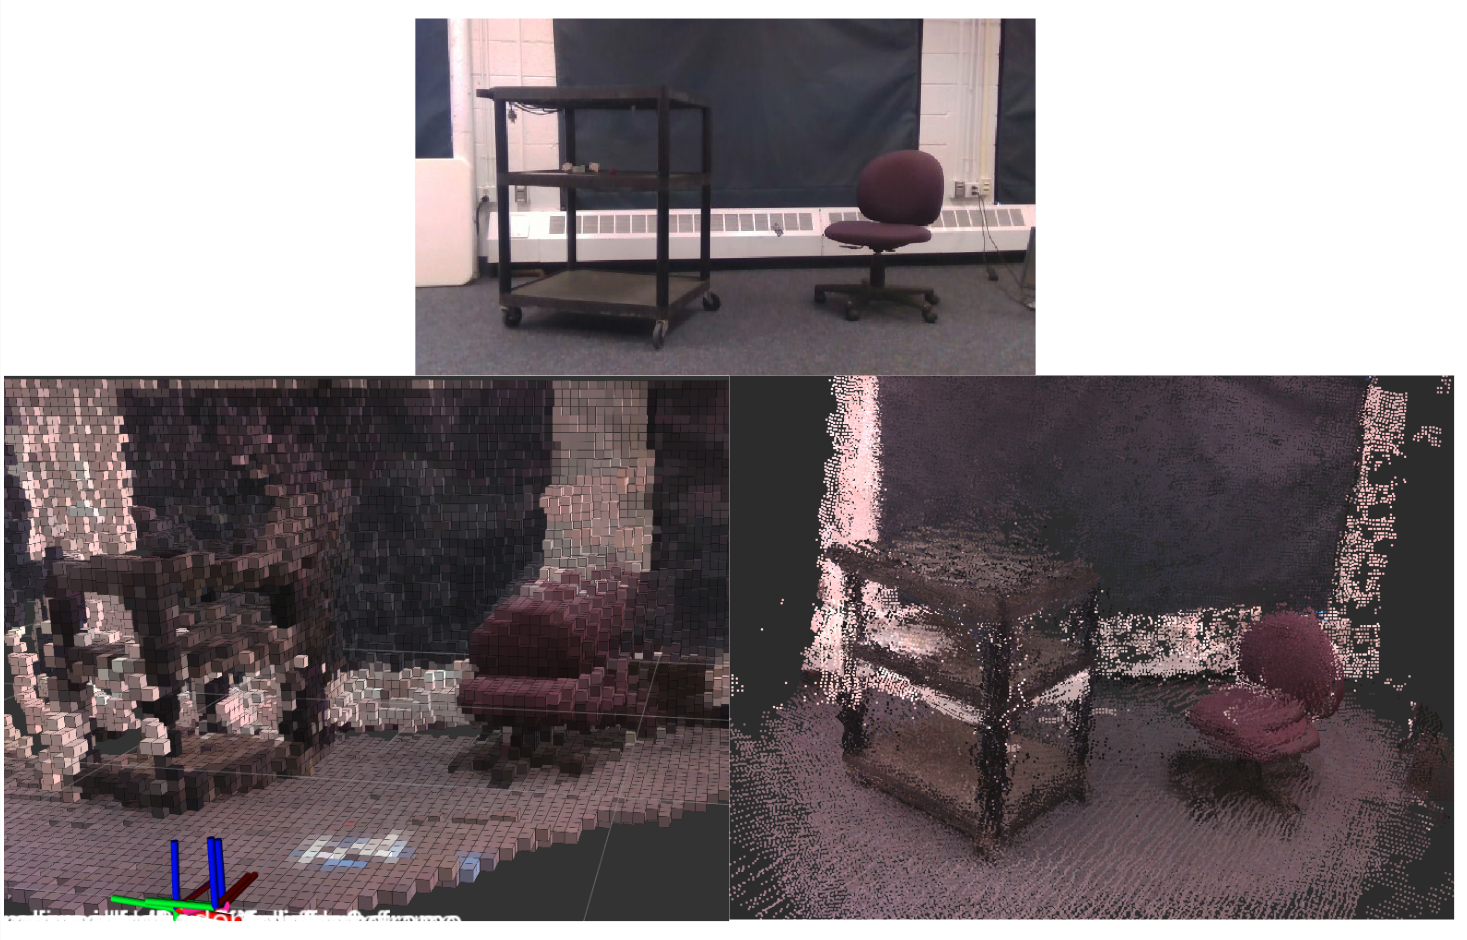
\includegraphics[trim = 0mm 0mm 0mm 0mm,clip,width=6.5in]{voxel.png}
	\caption{Comparison between an image(top), an octomap(left), and a pointcloud(right)}
	\label{fig:voxel}
\end{figure}

Over the last few years, 3D mapping technology has greatly improved. Labbe et al. \cite{Labbe2011a} \cite{Labbe2013} have developed a capable ROS package called RTAB-Map designed for creating 3D maps from RGB-D cameras. This package simplifies the problem of creating reliable 3D maps and is able to generate both point clouds and octomaps. It is also able to mesh multiple maps together into a single map using loop closures. It currently lacks the framework to build maps with multiple UAVs simultaneously.

Because of the limited flight durations of multirotor UAVs, when mapping areas that are larger than a single UAV can map in a flight, effectively merging maps from multiple agents into a single map is essential. Mangelson et al. \cite{Mangelson2018} recently derived a way to robustly merge multiple maps from a factor graph SLAM approach. They also discuss how this merging can happen real-time and improvements it makes over other methods of merging multiple maps.

In 2012 Micheal et al. \cite{Michael2012} tackled some of the collaborative mapping problem by using ground and aerial robots to collaboratively map an earthquake-damaged building. They used a LiDAR scanner and an RGB-D camera and mapped the building using a voxel grid. They were able to successfully merge the maps into a single well-structured map. Their results lacked simultaneous mapping and a sufficient map resolution to be used effectively by search and rescue teams.   

More recently in 2013, Zou et al. \cite{Zou2013} performed collaborative simultaneous SLAM with multiple handheld cameras to generate a single map and localize all agents on the map. In 2017, Schmuck et al. \cite{Schmuck2017} implemented monocular SLAM using multiple UAVs with downward facing cameras flying simultaneously to create a single shared map. Both of these instances successfully showed that it is possible for multiple agents to simultaneously generate a shared map. This research will be a good stepping stone, but it is different than the goal of this research project in that the map produced by the agents was sparse and would not be useful to first responders assessing the situation. 

\subsection{Planning}
In 2007 Bryson et al. \cite{Bryson2007} demonstrated the ability to plan multiple flight paths and navigate an area using multiple UAVs flying concurrently using an EKF-SLAM (extended Kalman filter SLAM) algorithm. This research was successful in having multiple agents find the same landmarks and create a single landmark map used to localize all UAVs. This research was done outdoors, not in a GPS-denied environment, and it was a landmark-based EKF-SLAM. The resulting map is only the landmark locations, generating only a sparse representation of the environment. This project aims to generate a dense, detailed representation of the environment that will be useful to first responders.

The path planning for this project will have the focus of generating flight paths that produce a sufficient map of the environment for humans to act upon the information in the map. In 2015 Martin et al. \cite{Martin2015} tackled a similar problem by using genetic algorithms to optimize flight paths that were able to effectively map uneven terrain and generate much more accurate maps than standard grid search flight paths. A similar approach to this will be used to plan efficient flight paths that are able to provide detailed, accurate maps of the indoor environment. 

From this brief survey of the current research, it can be seen that although various and significant contributions have been made in the field of collaborative planning and mapping, there is still great opportunity for continued research.  The research I am proposing will help to move some of the current research from the single UAV platforms to intelligent swarm applications, and help make the maps generated by these intelligent swarms more usable by humans.

\section{Research Objectives}

In completing the proposed research, the following objectives will be accomplished:


\begin{itemize}
	
	\item Determine and implement a functional approach to mapping an environment with multiple agents that will be human-readable and provide sufficient information for action

	\item Develop (or implement) an efficient planning algorithm for a team of UAVs that determines the UAV flight paths to successfully map the full search area with sufficient loop closure to mesh maps in a GPS-denied environment. 

	\item Implement the solution in hardware on a team of multirotor UAVs to simultaneously explore and map a GPS-denied environment


\end{itemize}

\section{Proposed Research}

To address the research, a multi-phase approach will be used. Research will commence by first setting up a simulation environment in ROS Gazebo to allow for frequent testing without relying on hardware every step of the way. Once the environment is set up, the project will be broken into three milestone hardware demonstrations: 

\subsection{Phase 1}
The first demonstration will be flying a single UAV in a GPS-denied environment to collect data and map the area. To complete this demonstration, an algorithm will be developed and implemented to plan the path in 3D space based off of a CAD model, a pre-made map, or blueprints of the search area. This path will be adjusted when unexpected obstacles and changes from the initial plans are detected. Although using an accurate odometry algorithm is essential to the success of this project, there are other students who are focusing on that aspect. In this phase, research will be done to determine a functional mapping algorithm for this scenario. It will then be implemented on the UAV to map the environment. 

\subsection{Phase 2}
The second phase of the project will be to get a single UAV to fly multiple paths in the same environment and mesh the maps into a single map. These paths will need to be optimized such that they cover the desired search area and overlap enough to provide sufficient loop closure to mesh the maps together in post processing. The goal of this optimization will be to generate flight paths for the UAV such that a sufficient map of the search area is created with the least amount of flight time possible. This phase will first be done with software simulation, then on hardware. This is where the bulk of novel research will be done. As mentioned earlier, because of the limited flight time of the multirotor UAVs, efficient flight paths will make the searching and mapping of large areas feasible.

\subsection{Phase 3}
The third and final phase of the project will be to get multiple UAVs flying simultaneously in the same environment and meshing the maps into a single map. This will require more effort on the path planning to make sure the paths can be flown simultaneously. Then the data will be sent to a more powerful off-board computer to make the map meshing as close to real time as possible. 


\section{Anticipated Contributions}

As a result of this research, there will be an improved method for exploring and mapping a GPS-denied environment with multiple UAVs, by developing the method for meshing a single map from multiple smaller maps. This process will also be streamlined to allow for near-real-time use of the maps by first responders. The goal is to publish this research in one relevant conference such as ICUAS (International Conference on Unmanned Aircraft Systems) or IROS (Intelligent Robots and Systems) about meshing multiple maps into a single map, and one relevant journal such as Journal of Intelligent and Autonomous Systems or Journal of Autonomous Robots about optimal simultaneous path planning for generating detailed maps. 

\pagebreak

\bibliographystyle{IEEEtran}
\bibliography{library}

\end{document}